\documentclass[12pt,a4paper]{article}
\usepackage[UTF8]{ctex}
\usepackage{amsmath,amssymb}
\usepackage{listings}
\usepackage{xcolor}
\usepackage{hyperref}
\usepackage{geometry}
\usepackage{graphicx}
\geometry{margin=2.5cm}

\lstdefinestyle{python}{
  language=Python,
  basicstyle=\ttfamily\small,
  keywordstyle=\color{blue}\bfseries,
  commentstyle=\color{gray},
  stringstyle=\color{red},
  showstringspaces=false,
  breaklines=true,
  frame=single,
  backgroundcolor=\color{gray!10}
}

\title{Simon's Algorithm / Simon 算法}
\author{QuoNic}
\date{}

\begin{document}
\maketitle

\begin{center}
\textbf{Algorithms / 算法} | 难度：高级 | 预计时间：15 分钟
\end{center}

\tableofcontents
\newpage

%% ============================================================
\section{为什么需要？}

Simon 算法是第一个证明量子指数加速的算法，是 Shor 算法的前身。

\subsection{经典局限}
\b\begin{itemize}
  \item 经典算法需要 $O(2^{n/2})$ 次查询
  \item 对于 $n$ 量子比特，经典需要指数次查询
\end{itemize}

\subsection{量子优势}
\b\begin{itemize}
  \item Simon 算法只需要 $O(n)$ 次查询
  \item 提供指数加速
  \item 是 Shor 算法的基础
\end{itemize}

\subsection{实际应用}
\b\begin{itemize}
  \item 量子算法设计
  \item Shor 算法（大数分解）
  \item 量子计算理论
\end{itemize}

%% ============================================================
\section{快速上手}

\begin{lstlisting}[style=python]
from quonic.algorithms import simon

# Find hidden period
result = simon("101", n_qubits=3)
print(f"Hidden period: {result.period}")
\end{lstlisting}

\textbf{预期输出}：
\begin{verbatim}
Hidden period: 101
\end{verbatim}

%% ============================================================
\section{原理详解}

\subsection{电路图}

\begin{center}
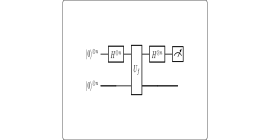
\includegraphics[width=0.6\textwidth]{../../images/simon_circuit.svg}
\end{center}

\subsection{数学推导}

Simon 算法寻找函数 $f$ 的隐藏周期 $s$，使得 $f(x) = f(x \oplus s)$。

\textbf{Step 1: 初始化}
\begin{equation}
|\psi_0\rangle = |0\rangle^{\otimes n}|0\rangle^{\otimes n}
\end{equation}

\textbf{Step 2: Hadamard 门}
\begin{equation}
|\psi_1\rangle = \frac{1}{\sqrt{2^n}} \sum_{x=0}^{2^n-1} |x\rangle|0\rangle
\end{equation}

\textbf{Step 3: Oracle 查询}
\begin{equation}
|\psi_2\rangle = \frac{1}{\sqrt{2^n}} \sum_{x=0}^{2^n-1} |x\rangle|f(x)\rangle
\end{equation}

\textbf{Step 4: 测量和后处理}

测量第二个寄存器，得到 $f(x)$。对第一个寄存器施加 Hadamard 门，测量得到 $y$，使得 $y \cdot s = 0 \mod 2$。

通过多次运行，收集足够的方程，求解得到 $s$。

\subsection{几何解释}

Simon 算法利用量子叠加态同时查询所有输入，通过干涉效应提取隐藏的周期信息。

%% ============================================================
\section{代码详解}

\begin{lstlisting}[style=python]
from quonic.algorithms import simon

# simon(period, n_qubits)
# period: the hidden period to find
# n_qubits: number of qubits
result = simon("101", n_qubits=3)

# result.period: the found period
print(f"Hidden period: {result.period}")
\end{lstlisting}

%% ============================================================
\section{进阶用法}

\subsection{场景 1：不同周期}

\begin{lstlisting}[style=python]
# Find different periods
result = simon("110", n_qubits=3)
print(f"Hidden period: {result.period}")
# Output: 110
\end{lstlisting}

\subsection{场景 2：多量子比特}

\begin{lstlisting}[style=python]
# More qubits for longer periods
result = simon("10110", n_qubits=5)
print(f"Hidden period: {result.period}")
# Output: 10110
\end{lstlisting}

%% ============================================================
\section{适用场景}

\subsection{量子算法设计}

Simon 算法是量子算法设计的范例。

\subsection{Shor 算法}

Simon 算法是 Shor 算法的前身。

\subsection{量子计算理论}

Simon 算法是量子计算理论的重要组成部分。

%% ============================================================
\section{常见问题}

\subsection{Simon 算法的加速比是多少？}

指数加速：经典需要 $O(2^{n/2})$ 次查询，量子只需要 $O(n)$ 次。

\subsection{Simon 算法和 Shor 算法有什么关系？}

Simon 算法是 Shor 算法的前身。Shor 算法将 Simon 算法推广到周期查找问题。

\subsection{Simon 算法的局限性是什么？}

Simon 算法只能处理二进制周期，不能处理一般的周期问题。

%% ============================================================
\section{学习路径}

\subsection{前置知识}
\b\begin{itemize}
  \item Deutsch-Jozsa 算法
  \item 量子比特和叠加态
  \item Hadamard 门和 CNOT 门
\end{itemize}

\subsection{继续学习}
\b\begin{itemize}
  \item Shor 算法
  \item 量子算法设计
  \item 量子计算理论
\end{itemize}

%% ============================================================
\section{完整示例代码}

\subsection{示例 1：基本 Simon 算法}

\begin{lstlisting}[style=python]
from quonic.algorithms import simon

result = simon("101", n_qubits=3)
print(f"Hidden period: {result.period}")
\end{lstlisting}


\section{下载}

\begin{itemize}
  \item [simon.py](https://github.com/ChrisLee0721/QuoNic/blob/main/examples/simon/simon.py)
\end{itemize}

\end{document}
